% **************************************************************************************************************
% A Classic Thesis Style
% An Homage to The Elements of Typographic Style
%
% Copyright (C) 2012 Andr\'e Miede http://www.miede.de
%
% If you like the style then I would appreciate a postcard. My address 
% can be found in the file ClassicThesis.pdf. A collection of the 
% postcards I received so far is available online at 
% http://postcards.miede.de
%
% License:
% This program is free software; you can redistribute it and/or modify
% it under the terms of the GNU General Public License as published by
% the Free Software Foundation; either version 2 of the License, or
% (at your option) any later version.
%
% This program is distributed in the hope that it will be useful,
% but WITHOUT ANY WARRANTY; without even the implied warranty of
% MERCHANTABILITY or FITNESS FOR A PARTICULAR PURPOSE.  See the
% GNU General Public License for more details.
%
% You should have received a copy of the GNU General Public License
% along with this program; see the file COPYING.  If not, write to
% the Free Software Foundation, Inc., 59 Temple Place - Suite 330,
% Boston, MA 02111-1307, USA.
%
% **************************************************************************************************************
% Note:
%    * You must not use "u etc. in strings/commands that will be spaced out (use \"u or real umlauts instead)
%    * New enumeration (small caps): \begin{aenumerate} \end{aenumerate}
%    * For margin notes: \marginpar or \graffito{}
%    * Do not use bold fonts in this style, it is designed around them
%    * Use tables as in the examples
%    * See classicthesis-preamble.sty for useful commands
% **************************************************************************************************************
% To Do:
%		 * [high] Check this out: http://www.golatex.de/koma-script-warnung-in-verbindung-mit-listings-package-t2058.html
%    * [medium] mathbb in section-titles/chapter-titles => disappears somehow in headlines!!!
% **************************************************************************************************************
\documentclass[ twoside,openright,titlepage,numbers=noenddot,headinclude,%1headlines,% letterpaper a4paper
                footinclude=true,cleardoublepage=plain,abstractoff, % <--- obsolete, remove (todo)
                BCOR=5mm,paper=a4,fontsize=11pt,%11pt,a4paper,%
                portuguese,
                dottedtoc, % adicionar pontinhos na lista de conteúdos
                ]{scrreprt}


% UTF-8 support with latin9 (ISO-8859-9) = latin1+"Euro sign"
\PassOptionsToPackage{utf8}{inputenc}   
\usepackage{inputenc}  
 
% ****************************************************************************************************
% Personal data and user ad-hoc commands
% ****************************************************************************************************
\newcommand{\myTitle}{Análise de ciber segurança ao Chromecast\xspace}
\newcommand{\myDegree}{Mestrado em Eng.ª Informática -- Computação Móvel\xspace}
\newcommand{\myNameOne}{Estudante xxxxxx xxxxxx xxxxxx\xspace}
\newcommand{\myNumber}{yyyyyyyy}


\newcommand{\myProfOne}{Professor Doutor XXXX XXXXX XXXXX  \href{mailto:xxxxxx@ipleiria.pt}{(xxxxxx@ipleiria.pt)}\xspace}
% \newcommand{\myProfTwo}{Professor Doutor XXXX XXXXX XXXXX \href{mailto:xxxxxx@ipleiria.pt}{(xxxxxx@ipleiria.pt)}\xspace}

\newcommand{\myFaculty}{Instituto Politécnico de Leiria\xspace}
\newcommand{\mySchool}{Escola Superior de Tecnologia e Gestão\xspace}
\newcommand{\myDepartment}{Departamento de Engenharia Informática\xspace}
\newcommand{\myLocation}{Leiria\xspace}

\newcommand{\myTime}{Fevereiro de 2019\xspace}
\newcommand{\mySchoolYear}{2018 -- 2019\xspace}
\newcommand{\myVersion}{versão 0.0\xspace}            
                
                
%*******************************************************
% Note: Make all your adjustments in here
%*******************************************************
% ****************************************************************************************************
% classicthesis-config.tex 
% formerly known as loadpackages.sty, classicthesis-ldpkg.sty, and classicthesis-preamble.sty 
% Use it at the beginning of your ClassicThesis.tex, or as a LaTeX Preamble 
% in your ClassicThesis.{tex,lyx} with \input{classicthesis-config}
% ****************************************************************************************************  
% If you like the classicthesis, then I would appreciate a postcard. 
% My address can be found in the file ClassicThesis.pdf. A collection 
% of the postcards I received so far is available online at 
% http://postcards.miede.de
% ****************************************************************************************************

% ****************************************************************************************************
% 1. Configure classicthesis for your needs here, e.g., remove "drafting" below 
% in order to deactivate the time-stamp on the pages
% ****************************************************************************************************
\PassOptionsToPackage{
                    eulerchapternumbers,
                    drafting, % comentar para remover a linha com a versão
                    pdfspacing,
                    %floatperchapter,
                    %linedheaders,%
                    subfig,beramono,
                    eulermath,
                    parts
                    }{classicthesis}
% Available options for classicthesis.sty 
% (see ClassicThesis.pdf for more information):
% drafting
% parts nochapters linedheaders
% eulerchapternumbers beramono eulermath pdfspacing minionprospacing
% tocaligned dottedtoc manychapters
% listings floatperchapter subfig
% ********************************************************************

% ********************************************************************
% Triggers for this config
% ******************************************************************** 
\usepackage{ifthen}
\newboolean{enable-backrefs} % enable backrefs in the bibliography
\setboolean{enable-backrefs}{false} % true false
% ****************************************************************************************************


% ********************************************************************
% Setup, finetuning, and useful commands
% ********************************************************************
\newcounter{dummy} % necessary for correct hyperlinks (to index, bib, etc.)
\newlength{\abcd} % for ab..z string length calculation
\providecommand{\mLyX}{L\kern-.1667em\lower.25em\hbox{Y}\kern-.125emX\@}
\newcommand{\ie}{\textit{i.\,e.}\xspace}
\newcommand{\Ie}{\textit{I.\,e.}\xspace}
\newcommand{\eg}{\textit{e.\,g.}\xspace}
\newcommand{\Eg}{\textit{E.\,g.}\xspace} 
\newcommand{\etc}{\textit{etc}\xspace} 


% ****************************************************************************************************
% \DeclareTextFontCommand{\code}{\fontfamily{pcr}\scriptsize}


% ****************************************************************************************************
% 3. Loading some handy packages
% ****************************************************************************************************
% ******************************************************************** 
% Packages with options that might require adjustments
% ******************************************************************** 

\PassOptionsToPackage{portuguese}{babel}
\usepackage{babel}

 
%%%%%%%%%%%%%%%%%%%%%%%%%%%%%%%%%%%%%%%%%%%%%%%%%%%%%
% Bibliografia
%%%%%%%%%%%%%%%%%%%%%%%%%%%%%%%%%%%%%%%%%%%%%%%%%%%%%
% package recomendada para usar com o biblatex
\usepackage{csquotes}

% carrega a package biblatex
\usepackage[
    backend=biber,    % usar o biber para processar
    style=authoryear, % estilo de citação
    sortcites=true,
    maxcitenames=2,   % a partir de 2 escreve "et al."
]{biblatex} 

% para adicionar uma vírgula antes do ano: (Dirac, 1981)
\renewcommand*{\nameyeardelim}{\addcomma\space}

%  dica: configurar o kile para reconhecer os comandos:
%    \parencite{bibkey}
%    \textcite{bibkey}
%    \citeauthor{bibkey}
%    \citetitle{bibkey}
%    
%    Settingis -> Configure Kile -> Latex/General -> Commands/Configure -> Commands/Citation -> add
%%%%%%%%%%%%%%%%%%%%%%%%%%%%%%%%%%%%%%%%%%%%%%%%%%%%%
 
\usepackage{float}

\PassOptionsToPackage{fleqn}{amsmath}		% math environments and more by the AMS 
\usepackage{amsmath}

\usepackage{multirow}
 
%******************************************************************** 
% General useful packages
%******************************************************************** 
\PassOptionsToPackage{T1}{fontenc} % T2A for cyrillics
\usepackage{fontenc}

\usepackage{textcomp} % fix warning with missing font shapes
\usepackage{scrhack} % fix warnings when using KOMA with listings package          
\usepackage{xspace} % to get the spacing after macros right  
\usepackage{mparhack} % get marginpar right
% \usepackage{fixltx2e} % fixes some LaTeX stuff 

\PassOptionsToPackage{printonlyused,smaller}{acronym}
\usepackage{acronym} % nice macros for handling all acronyms in the thesis

%\renewcommand*{\acsfont}[1]{\textssc{#1}} % for MinionPro
\newcommand{\bflabel}[1]{{#1}\hfill} % fix the list of acronyms
%****************************************************************************************************


%****************************************************************************************************
% 4. Setup floats: tables, (sub)figures, and captions
%****************************************************************************************************
\usepackage{tabularx} % better tables
    \setlength{\extrarowheight}{3pt} % increase table row height
\newcommand{\tableheadline}[1]{\multicolumn{1}{c}{\spacedlowsmallcaps{#1}}}
\newcommand{\tableheadlineR}[1]{\multicolumn{1}{r}{\spacedlowsmallcaps{#1}}}
\newcommand{\myfloatalign}{\centering} % to be used with each float for alignment
\usepackage{caption}
\captionsetup{format=hang,font=small}
\usepackage{subfig}  
% ****************************************************************************************************


%----------------------------------------------------------
% Filipius's famous "issue" command (Patricio, 2016-08-03)
%----------------------------------------------------------
\newcommand{\issue}[1] { {\footnotesize\textbf{
    \begin{center}
      \begin{tabular}{|c|}
        \hline
	\parbox[c]{\textwidth}{
          \medskip
          #1
          \medskip} \\
        \hline
      \end{tabular}
    \end{center}
  }
 }
}


% ****************************************************************************************************
% 6. PDFLaTeX, hyperreferences and citation backreferences
% ****************************************************************************************************
% ********************************************************************
% Using PDFLaTeX
% ********************************************************************
\PassOptionsToPackage{pdftex,hyperfootnotes=false,pdfpagelabels}{hyperref}
	\usepackage{hyperref}  % backref linktocpage pagebackref
\pdfcompresslevel=9
\pdfadjustspacing=1 
\PassOptionsToPackage{pdftex}{graphicx}
	\usepackage{graphicx} 

% ********************************************************************
% Setup the style of the backrefs from the bibliography
% (translate the options to any language you use)
% ********************************************************************
\newcommand{\backrefnotcitedstring}{\relax}%(Not cited.)
\newcommand{\backrefcitedsinglestring}[1]{(Cited on page~#1.)}
\newcommand{\backrefcitedmultistring}[1]{(Cited on pages~#1.)}
\ifthenelse{\boolean{enable-backrefs}}%
{%
		\PassOptionsToPackage{hyperpageref}{backref}
		\usepackage{backref} % to be loaded after hyperref package 
		   \renewcommand{\backreftwosep}{ and~} % separate 2 pages
		   \renewcommand{\backreflastsep}{, and~} % separate last of longer list
		   \renewcommand*{\backref}[1]{}  % disable standard
		   \renewcommand*{\backrefalt}[4]{% detailed backref
		      \ifcase #1 %
		         \backrefnotcitedstring%
		      \or%
		         \backrefcitedsinglestring{#2}%
		      \else%
		         \backrefcitedmultistring{#2}%
		      \fi}%
}{\relax}    

% ********************************************************************
% Hyperreferences
% ********************************************************************
\hypersetup{%
    %draft,	% = no hyperlinking at all (useful in b/w printouts)
    colorlinks=true, linktocpage=true, pdfstartpage=3, pdfstartview=FitV,%
    % uncomment the following line if you want to have black links (e.g., for printing)
    %colorlinks=false, linktocpage=false, pdfborder={0 0 0}, pdfstartpage=3, pdfstartview=FitV,% 
    breaklinks=true, pdfpagemode=UseNone, pageanchor=true, pdfpagemode=UseOutlines,%
    plainpages=false, bookmarksnumbered, bookmarksopen=true, bookmarksopenlevel=1,%
    hypertexnames=true, pdfhighlight=/O,%nesting=true,%frenchlinks,%
    urlcolor=RoyalBlue, linkcolor=RoyalBlue, citecolor=RoyalBlue, %pagecolor=RoyalBlue,%
    %urlcolor=Black, linkcolor=Black, citecolor=Black, %pagecolor=Black,%
    pdftitle={\myTitle},%
    pdfauthor={\textcopyright\ \myNameOne, \myDegree, \myDepartment, \mySchool, \myFaculty},%
    pdfsubject={},%
    pdfkeywords={},%
    pdfcreator={pdfLaTeX},%
    pdfproducer={LaTeX with hyperref and classicthesis}%
}   

% ********************************************************************
% Setup autoreferences
% ********************************************************************
% There are some issues regarding autorefnames
% http://www.ureader.de/msg/136221647.aspx
% http://www.tex.ac.uk/cgi-bin/texfaq2html?label=latexwords
% you have to redefine the makros for the 
% language you use, e.g., american, ngerman
% (as chosen when loading babel/AtBeginDocument)
% ********************************************************************
\makeatletter
\@ifpackageloaded{babel}%
    {%
       \addto\extrasamerican{%
					\renewcommand*{\figureautorefname}{Figure}%
					\renewcommand*{\tableautorefname}{Table}%
					\renewcommand*{\partautorefname}{Part}%
					\renewcommand*{\chapterautorefname}{Chapter}%
					\renewcommand*{\sectionautorefname}{Section}%
					\renewcommand*{\subsectionautorefname}{Section}%
					\renewcommand*{\subsubsectionautorefname}{Section}% 	
				}%
       \addto\extrasngerman{% 
					\renewcommand*{\paragraphautorefname}{Absatz}%
					\renewcommand*{\subparagraphautorefname}{Unterabsatz}%
					\renewcommand*{\footnoteautorefname}{Fu\"snote}%
					\renewcommand*{\FancyVerbLineautorefname}{Zeile}%
					\renewcommand*{\theoremautorefname}{Theorem}%
					\renewcommand*{\appendixautorefname}{Anhang}%
					\renewcommand*{\equationautorefname}{Gleichung}%        
					\renewcommand*{\itemautorefname}{Punkt}%
				}%	
			% Fix to getting autorefs for subfigures right (thanks to Belinda Vogt for changing the definition)
			\providecommand{\subfigureautorefname}{\figureautorefname}%  			
    }{\relax}
\makeatother


% ****************************************************************************************************
% 7. Last calls before the bar closes
% ****************************************************************************************************
% ********************************************************************
% Development Stuff
% ********************************************************************
\listfiles
%\PassOptionsToPackage{l2tabu,orthodox,abort}{nag}
%	\usepackage{nag}
%\PassOptionsToPackage{warning, all}{onlyamsmath}
%	\usepackage{onlyamsmath}


% ********************************************************************
% Last, but not least...
% ********************************************************************
\usepackage{classicthesis} 
% ****************************************************************************************************


\clearscrheadfoot
\ohead[]{\headmark}
\ofoot[\pagemark]{\pagemark}

% incluir PDFs
\usepackage{pdfpages}

% ****************************************************************************************************
% 8. Further adjustments (experimental)
% ****************************************************************************************************

\usepackage{setspace}

% recomendado por ser o mais próximo do word
\spacing{1.3}


% ********************************************************************
% Changing the text area
% ********************************************************************
%\linespread{1.05} % a bit more for Palatino
%\areaset[current]{312pt}{761pt} % 686 (factor 2.2) + 33 head + 42 head \the\footskip
%\setlength{\marginparwidth}{7em}%
%\setlength{\marginparsep}{2em}%

% ********************************************************************
% Using different fonts
% ********************************************************************
%\usepackage[oldstylenums]{kpfonts} % oldstyle notextcomp
%\usepackage[osf]{libertine}
%\usepackage{hfoldsty} % Computer Modern with osf
%\usepackage[light,condensed,math]{iwona}
%\renewcommand{\sfdefault}{iwona}
\usepackage{lmodern} % <-- no osf support :-(
%\usepackage[urw-garamond]{mathdesign} <-- no osf support :-(
% ****************************************************************************************************

% \usepackage{inconsolata}

\usepackage{caption}
% \usepackage{caption,setspace}
% \captionsetup[lstlisting]{belowskip=0pt}
% \captionsetup[lstlisting]{belowcaptionskip=0pt}
% \captionsetup[lstinputlisting]{belowcaptionskip=0pt}
% \captionsetup[listing]{font={stretch=0.8}}


% o mint dá erro se pedirmos para imprimir o @
\newcommand{\at}{\makeatletter @\makeatother}



%%%%%%%%%%%%%%%%%%%%%%%%%%%%%%%%%%%%%%%%%%%%%%%%%%%%%%%%%%%%%%%%%%%%%%%%%%
% INÍCIO minted --- colorir código fonte
%%%%%%%%%%%%%%%%%%%%%%%%%%%%%%%%%%%%%%%%%%%%%%%%%%%%%%%%%%%%%%%%%%%%%%%%%%


\usepackage[newfloat]{minted}	% package responsável pelo processamento

\SetupFloatingEnvironment{listing}{name=Listagem, within=none}
\captionsetup[listing]{position=above,skip=-3pt} % remover espaço vertical demasiado grande

% criar ambiente para listagem de código que ocupa mais de uma página.
\newenvironment{longlisting}{
        \bigskip\medskip
        \captionsetup{type=listing}
    }{
        \bigbreak
        \medskip
    }


% estilo pré-definido, fazer: pygmentize -L style para ver mais estilos
\usemintedstyle{autumn} 

% definir estilos
% 
% NOTA:
% 	para o kile reconhecer este estilo, tive de editar o ficheiro
% 	sudo vim /usr/share/kde4/apps/katepart/syntax/latex.xml
% 	e acrescentar: 
% 	<!-- mfrade -->
%         <StringDetect String="bashcode" attribute="Environment" context="MintedEnvParam"/>
% 
% 	e depois adicionar "|bashcode" sempre que aparecia "minted" no ficheiro, ex.
% 	<RegExpr String="\\end\s*\{(lstlisting|minted|bashcode)\*?\}"

\newmint{bash}{
  fontsize=\scriptsize,
  fontfamily=courier,
  linenos=false
}

\newminted{python}{
  frame=lines,
  framesep=2mm,
  fontsize=\scriptsize,
  fontfamily=courier,
  linenos=true,
  breaklines=true,
  breakanywhere=true,
}

\newmintedfile[codefilec]{c}{
  frame=lines,
  framesep=2mm,
  fontsize=\scriptsize,
  fontfamily=courier,
  linenos=true,
  breaklines=true,
  breakanywhere=true,
}

\newmintedfile[codefilebash]{bash}{
  frame=lines,
  framesep=2mm,
  fontsize=\scriptsize,
  fontfamily=courier,
  linenos=true,
  breaklines=true,
  breakanywhere=true,
}

% \newmintinline[code]{text}{fontsize=\footnotesize,fontfamily=courier}
\newmintinline[code]{text}{fontsize=\footnotesize,fontfamily=tt}

% mudar o aspeto da numeração
\renewcommand{\theFancyVerbLine}{\tiny\ttfamily%
  \textcolor[rgb]{0.7,0.7,0.7}{\arabic{FancyVerbLine}}%
}

%%%%%%%%%%%%%%%%%%%%%%%%%%%%%%%%%%%%%%%%%%%%%%%%%%%%%%%%%%%%%%%%%%%%%%%%%%
% FIM --- minted
%%%%%%%%%%%%%%%%%%%%%%%%%%%%%%%%%%%%%%%%%%%%%%%%%%%%%%%%%%%%%%%%%%%%%%%%%%

% controlar o tamanho das margens
% \usepackage{showframe}
\marginparwidth=0pt
\marginparsep=5pt
\addtolength{\evensidemargin}{-15mm}
\addtolength{\textwidth}{20mm}

% espaçamento entre parágrafos
\setlength{\parskip}{0.5em}

% obter o símbolo do Euro
\usepackage{eurosym}
\DeclareUnicodeCharacter{20AC}{\euro} % aceita o símbolo do teclado
% usar a vírgula como separador decimal
\usepackage{icomma}

% 
% tem de ser carregada depois do hyperref
% 
\PassOptionsToPackage{xindy,style=super,nolist}{glossaries}
\PassOptionsToPackage{acronym}{glossaries}
\PassOptionsToPackage{nonumberlist}{glossaries}
\usepackage{glossaries}


% avoid numbering empty pages
\usepackage{emptypage}


% permite quebrar a 1ª coluna
\newglossarystyle{clong}{%
 \renewenvironment{theglossary}%
%      {\begin{longtable}{p{.2\linewidth}p{\glsdescwidth}}}%
     {\begin{longtable}{p{.18\linewidth}p{.78\linewidth}}}%
     {\end{longtable}}%
  \renewcommand*{\glossaryheader}{}%
  \renewcommand*{\glsgroupheading}[1]{}%
  \renewcommand*{\glossaryentryfield}[5]{%
    \glstarget{##1}{##2} & ##3\glspostdescription\space ##5\\}%
  \renewcommand*{\glossarysubentryfield}[6]{%
     & \glstarget{##2}{\strut}##4\glspostdescription\space ##6\\}%
  %\renewcommand*{\glsgroupskip}{ & \\}%
}


\usepackage{lipsum}

%*******************************************************
% Bibliography
%*******************************************************
%   Ficheiro com a base de dados da bibliografia
\addbibresource{References.bib}
%   para o kile dar as sugestões das chaves da bibliografia
%   se der erro a queixar-se do bibtex, basta repetir a compilação
\iffalse
    \bibliography{References.bib}  % só para o kile
\fi


%*******************************************************
% Lista de acrónimos
%*******************************************************
% \loadglsentries{Covers/Acronyms-list}
\makeglossaries


%*******************************************************
% Hyphenation
%*******************************************************
%\hyphenation{put special hyphenation here}


% ******************************************************
% GO!GO!GO! MOVE IT!
%*******************************************************
\begin{document}
\frenchspacing
\raggedbottom
\selectlanguage{portuguese}

\pagestyle{plain}

% use \cleardoublepage here to avoid problems with pdfbookmark

%*******************************************************
% Frontmatter
%*******************************************************
% Title Page

\begin{titlepage}

\begin{center}
\large

\hfill

% \includegraphics[width=8cm]{Covers/ipl-estg} \\

\includegraphics[width=\textwidth]{Covers/estg_h.png} \\


\bigskip
\myFaculty \\
\mySchool \\ 
\myDepartment \\
\myDegree \\



\begingroup
\color{Maroon}

\vspace{4cm}

\spacedallcaps{\myTitle} \\ \bigskip % Thesis title
\endgroup
% \mySubtitle \\ \medskip % Thesis subtitle

\vspace{4cm}

% \vfill


\spacedlowsmallcaps{\myNameOne} \\
% \spacedlowsmallcaps{\myNameTwo}
\bigskip % Your name

\vfill


\myLocation, \myTime\ %-- \myVersion % Time and version



\end{center}
% \end{addmargin}

\end{titlepage}


\cleardoublepage% Title Page

\begin{titlepage}

\begin{center}

\hfill

% \includegraphics[width=8cm]{Covers/ipl-estg} \\

\includegraphics[width=\textwidth]{Covers/estg_h.png} \\

\bigskip
\large
\myFaculty \\
\mySchool \\ 
\myDepartment \\
\myDegree \\



\begingroup
\color{Maroon}

\vspace{4cm}

\spacedallcaps{\myTitle} \\ \bigskip % Thesis title
\endgroup
% \mySubtitle \\ \medskip % Thesis subtitle

\vspace{4cm}

% \vfill


\spacedlowsmallcaps{\myNameOne}\\
Número: \myNumber \\
% \spacedlowsmallcaps{\myNameTwo}
\bigskip % Your name

\vfill

\end{center}

\begin{normalsize}
    
    \noindent Dissertação realizada sob orientação do \myProfOne.

\end{normalsize}
\vspace{1cm}

\begin{center}

\myLocation, \myTime\ %-- \myVersion % Time and version
    
\end{center}



% \end{addmargin}

\end{titlepage}

\cleardoublepage



\pagenumbering{roman}
\cleardoublepage%*******************************************************
% Acknowledgments
%*******************************************************


\refstepcounter{dummy}
\addcontentsline{toc}{chapter}{Agradecimentos}

% \begin{flushright}{\slshape    
%     We have seen that computer programming is an art, \\ 
%     because it applies accumulated knowledge to the world, \\ 
%     because it requires skill and ingenuity, and especially \\
%     because it produces objects of beauty.} \\ \medskip
%     --- Donald Knuth
% \end{flushright}
% 
% 
% 
% \bigskip

\begingroup
\let\clearpage\relax
\let\cleardoublepage\relax
\let\cleardoublepage\relax
\chapter*{Agradecimentos}
Colocar os  agradecimentos aqui.

Agradeço ao meu orientador esta oportunidade de aprender a trabalhar em \LaTeXe.



\endgroup




\cleardoublepage%*******************************************************
% Abstract
%*******************************************************


\renewcommand{\abstractname}{Resumo}
\markboth{\spacedlowsmallcaps{\abstractname}}{\spacedlowsmallcaps{\abstractname}}
\refstepcounter{dummy}
\addcontentsline{toc}{chapter}{\abstractname}


\begingroup
\let\clearpage\relax
\let\cleardoublepage\relax
\let\cleardoublepage\relax

\chapter*{Resumo}
Um resumo deve conter uma breve descrição do problema do vosso projecto, da metodologia que utilizaram como estratégia para resolver esse problema, e dos principais resultados obtidos com o vosso trabalho. O resumo é sempre a última parte a ser escrita num relatório, ou tese.\\



\bigskip


\endgroup			

\cleardoublepage

\renewcommand{\abstractname}{Abstract}
\markboth{\spacedlowsmallcaps{\abstractname}}{\spacedlowsmallcaps{\abstractname}}
\refstepcounter{dummy}
\addcontentsline{toc}{chapter}{\abstractname}


\begingroup
\let\clearpage\relax
\let\cleardoublepage\relax
\let\cleardoublepage\relax

\chapter*{Abstract}
Escrever o resumo em Inglês.\\

\bigskip


\endgroup           


\pagestyle{scrheadings}

\cleardoublepage% Table of Contents - List of Tables/Figures/Listings and Acronyms

\refstepcounter{dummy}

\addcontentsline{toc}{chapter}{Índice}
% \pdfbookmark[1]{\contentsname}{tableofcontents} % Bookmark name visible in a PDF viewer

\setcounter{tocdepth}{2} % Depth of sections to include in the table of contents - currently up to subsections

\setcounter{secnumdepth}{3} % Depth of sections to number in the text itself - currently up to subsubsections

\renewcommand\contentsname{Índice}

\manualmark
\markboth{\spacedlowsmallcaps{\contentsname}}{\spacedlowsmallcaps{\contentsname}}
\tableofcontents 
\automark[section]{chapter}
\renewcommand{\chaptermark}[1]{\markboth{\spacedlowsmallcaps{#1}}{\spacedlowsmallcaps{#1}}}
\renewcommand{\sectionmark}[1]{\markright{\thesection\enspace\spacedlowsmallcaps{#1}}}

% \clearpage

\vspace*{8ex}
\newpage
\cleardoublepage

% \begingroup 
% \let\clearpage\relax
% \let\cleardoublepage\relax
% \let\cleardoublepage\relax

%----------------------------------------------------------------------------------------
%	List of Figures
%----------------------------------------------------------------------------------------

\refstepcounter{dummy}
\addcontentsline{toc}{chapter}{\listfigurename} % Uncomment if you would like the list of figures to appear in the table of contents
% \pdfbookmark[1]{\listfigurename}{lof} % Bookmark name visible in a PDF viewer

\listoffigures

\vspace*{8ex}
% \newpage
\cleardoublepage

%----------------------------------------------------------------------------------------
%	List of Tables
%----------------------------------------------------------------------------------------

% \phantomsection 
\refstepcounter{dummy}
\addcontentsline{toc}{chapter}{\listtablename} % Uncomment if you would like the list of tables to appear in the table of contents
% \pdfbookmark[1]{\listtablename}{lot} % Bookmark name visible in a PDF viewer

\listoftables

\clearpage

\vspace*{8ex}
% \newpage
% \cleardoublepage
    
%----------------------------------------------------------------------------------------
%	List of Listings
%---------------------------------------------------------------------------------------- 

% \refstepcounter{dummy}
% %\addcontentsline{toc}{chapter}{\lstlistlistingname} % Uncomment if you would like the list of listings to appear in the table of contents
% \pdfbookmark[1]{\lstlistlistingname}{lol} % Bookmark name visible in a PDF viewer
% 
% % \lstlistoflistings 
% 
% \vspace*{8ex}
% \newpage
       
% \endgroup



% %----------------------------------------------------------------------------------------
% %	Glossário
% %----------------------------------------------------------------------------------------
% 
% 
% \refstepcounter{dummy}
% \addcontentsline{toc}{chapter}{Glossário} % Uncomment if you would like the acronyms to appear in the table of contents
% % \pdfbookmark[1]{Lista de Acrónimos}{Lista de Acrónimos} % Bookmark name visible in a PDF viewer
% 
% 
% 
% \markboth{\spacedlowsmallcaps{Glossário}}{\spacedlowsmallcaps{Glossário}}
% \printglossary[type=\glsdefaulttype,title=Glossário]
% 
% 
% 
% 
% \cleardoublepage
\cleardoublepage%----------------------------------------------------------------------------------------
%   Acronyms
%----------------------------------------------------------------------------------------

\newacronym{dns}{DNS}{Domain Name System}
\newacronym{adsl}{ADSL}{Assimetric Digital Subscriber Line}
\newacronym{ascii}{ASCII}{American Standard Code for Information Interchange}
\newacronym{bios}{BIOS}{Basic Input/Output System}
\newacronym{bit}{bit}{Digito binário}
\newacronym{byte}{Byte}{Unidade de informação digital composta por oito bits}
\newacronym{cpu}{CPU}{Central Processing Unit}
\newacronym{codec}{CODEC}{COmpression/DECompression}
\newacronym{dll}{DLL}{Dynamic Link Library}
\newacronym{dhcp}{DHCP}{Dynamic Host Configuration Protocol}
\newacronym{ftp}{FTP}{File Transfer Protocol}
\newacronym{ip}{IP}{Internet Protocol}
\newacronym{isp}{ISP}{Internet Service Provider}
\newacronym{so}{SO}{Sistema Operativo}
\newacronym{tcp}{TCP}{Transmission Control Protocol}
\newacronym{abc}{ABC}{A lista de acrónimos deve ficar ordenada alfabeticamente}


%----------------------------------------------------------------------------------------
%   Formatação da página dos acrónimos
%----------------------------------------------------------------------------------------
\renewcommand{\acronymname}{Lista de Abreviaturas}
% \markboth{\spacedlowsmallcaps{\acronymname}}{\spacedlowsmallcaps{\acronymname}}
\refstepcounter{dummy}
\phantomsection 
\addcontentsline{toc}{chapter}{\acronymname}
% \addtocontents{toc}{\protect\vspace{\beforebibskip}} % to have the bib a bit from the rest in the toc

%  serve para eliminar quebras de página a mais
\begingroup
\let\clearpage\relax
\let\cleardoublepage\relax
\let\cleardoublepage\relax


\glsaddall

\printglossary[type=\acronymtype,style=super,title=\acronymname]

% as definições de abreviaturas estão no ficheiro
% 	Covers/Acronyms-list.tex


\endgroup	

\cleardoublepage



%********************************************************************
% Mainmatter
%*******************************************************
\pagenumbering{arabic}

% \phantomsection 
% \part*{Relatório}


\cleardoublepage\addtocontents{toc}{\protect\vspace{\beforebibskip}} % Place slightly below the rest of the document content in the table

%************************************************
\chapter{Introdução}
\label{ch:introduction}
%************************************************


Este documento serve de orientação para o relatório da unidade curricular de Projecto Informático do Curso de Engenharia Informática da ESTG – IPLEIRIA. Como tal, é constituído por um conjunto predefinido de estilos a utilizar. Estes estilos devem ser utilizados sem serem alterados ou substituídos. Para começar facilmente a escrever o relatório, basta guardar uma cópia deste documento e substituir os campos e as secções de acordo com o projecto em questão.

Embora possa parecer uma abordagem demasiadamente descritiva para a escrita do relatório, as intenções pretendidas com este documento são:

\begin{itemize}
 \item Focar os alunos na produção de conteúdos com qualidade, em vez de se preocuparem com formatações de tipos de letra, parágrafos, etc.;
 \item Ao fornecer um documento de orientação de estilos a Escola beneficia de um aspecto profissional e consistente da globalidade dos seus relatórios de projecto.
\end{itemize}


Quanto ao conteúdo de uma introdução, ele deve preparar o leitor para o resto do relatório. Deve conter o detalhe suficiente para que alguém das áreas de conhecimento envolvidas possa entender o assunto do trabalho. A maior parte das introduções contêm três partes para fornecer contexto ao trabalho: objectivos, âmbito e background do trabalho do projecto. Estas partes muitas vezes sobrepõem-se, e podem por vezes ser omitidas simplesmente porque não faz sentido incluir alguma delas.

É de extrema importância considerar os objectivos do trabalho e do relatório na introdução. Se os autores não entenderem bem os objectivos do trabalho, dificilmente o leitor os entenderá. As seguintes questões ajudam a pensar nos objectivos do trabalho e na razão da escrita do relatório:

\begin{enumerate}
 \item O que foi descoberto ou provado?
 \item Em que tipos de problemas se trabalhou?
 \item Porque é que se trabalhou nestes problemas? Se o problema lhe foi atribuído, deve tentar-se saber as razões pelas quais os orientadores o formularam, e o que era suposto que os alunos aprendessem ao trabalharem neste problema;
 \item Qual a razão da escrita deste relatório?
 \item O que é que o leitor deve ficar a saber quando acabar de ler este relatório?
\end{enumerate}


O âmbito deve indicar as áreas de conhecimento envolvidas e realçar a metodologia utilizada no trabalho de projecto. Referir o âmbito do projecto na introdução ajuda o leitor a perceber os parâmetros de entrada do trabalho e do relatório, bem como a identificar as principais restrições consideradas (por exemplo “existem 5 Sistemas Operativos para trabalhar com determinado hardware, mas somente 3 foram considerados neste estudo”). As seguintes questões ajudam a pensar no âmbito do trabalho e do relatório:

\begin{enumerate}
 \item De que forma foi abordado o problema, e qual a razão para tal abordagem?
 \item Existiam outras abordagens óbvias que se poderiam ter adoptado ? Que limitações impediram que se tentassem outras abordagens?
 \item Que factores contribuíram para a escolha da forma de como se abordou o problema, e qual o mais relevante nessa escolha?
\end{enumerate}

A informação de background inclui os conhecimentos que o leitor deve possuir por forma a compreender o trabalho de projecto e correspondente relatório. Estes conhecimentos incluem a percepção de trabalhos prévios que motivaram a proposta do projecto corrente, ou referências a trabalhos teóricos e práticos relacionados com os objectivos e âmbito descritos acima. Devem remeter-se para anexos documentos que poderão ajudar na percepção de teorias, metodologias, técnicas ou ferramentas utilizadas no trabalho de projecto. As seguintes questões ajudam a pensar no background necessário para o trabalho e para o relatório:

\begin{enumerate}
 \item Que factos deve o leitor conhecer para perceber o relatório?
 \item Porque é que o projecto foi autorizado ou atribuído?
 \item Quem já fez trabalho prévio para resolver o problema colocado pelo projecto?
\end{enumerate}

Por fim, a introdução deve descrever como foi organizado o relatório, referindo brevemente o propósito de cada secção considerada no mesmo.

O resto deste documento dá uma breve perspectiva das partes seguintes que devem constar do relatório, bem como de outros aspectos de formatação.

\cleardoublepage\addtocontents{toc}{\protect\vspace{\beforebibskip}} % Place slightly below the rest of the document content in the table

%************************************************
\chapter{Tabalho Relacionado}
\label{ch:background}
%************************************************


Escrever aqui tudo o que é trabalho relacionado com o projeto a ser desenvolvido. Neste capítulo as referências bibliográficas são extremamente importantes e podem ser feitas da seguinte forma (ver código fonte do \LaTeX): 

Para fazer uma citação no fim de uma frase: \parencite{Sims1992}. Multiplas citações \parencite{Darwin1859,Koza1992}

Para fazer uma citação que serve também como sujeito dessa frase (por exemplo no início): \textcite{Sims1992}

Obter apenas o nome do autor: \citeauthor{Sims1992}

Obter apenas o título do obra: \citetitle{Sims1992} 


Segundo \textcite{Rudolph2016} isto assim assado, bla .... \citetitle{Rudolph2016}


fgdfgdf
\begin{itemize}
    \item 1212
    \item dsafsdfds
    \item dsfdsf
\end{itemize}

sadsadsa
\begin{enumerate}
    \item asdsad
    \item sdfsfdsf
    \item dsfdsfds
\end{enumerate}


\cleardoublepage\addtocontents{toc}{\protect\vspace{\beforebibskip}} % Place slightly below the rest of the document content in the table


%************************************************
\chapter{Desenvolvimento}
\label{ch:desenvolvimento}
%************************************************


O corpo do relatório compõe, normalmente, a parte mais extensa do relatório, e contém todos os conteúdos necessários para que o leitor perceba o assunto do mesmo. Estes conteúdos incluem detalhes, dados, resultados de teste, factos e conclusões. O que incluir exactamente no corpo do relatório e como será organizado é determinado pelo contexto do trabalho desenvolvido. Geralmente, o corpo do relatório inclui 7 secções distintas:

\begin{enumerate}
 \item Uma secção para teorias, modelos e hipóteses. Esta secção tem uma maior proeminência em artigos de investigação, onde é sugerida uma hipótese (contribuição) inovadora. Esta secção deve ser omitida para o caso de trabalhos mais práticos, cuja elaboração não origine uma contribuição inovadora, mas sim num produto de aplicação de tecnologias e metodologias;
 \item Uma secção onde são discutidas as tecnologias, metodologias, ferramentas e técnicas utilizadas, e a forma como foram adequadas para se fazerem cumprir com os objectivos do trabalho. Algumas questões que esta secção deve procurar responder incluem:
 \begin{itemize}
  \item Que equipamentos de hardware e ferramentas de software foram utilizados para o desenvolvimento do trabalho?
  \item Qual a metodologia de desenvolvimento foi adoptada, e como é que ela se reflecte em termos de protótipos, modelos, diagramas, código, testes e documentação, de acordo com os objectivos do projecto? Sugere-se a utilização de exemplos no corpo do relatório, remetendo para anexos a descrição dos produtos intermédios completos;
  \item Como foi planeado o trabalho, em termos de sequenciamento de actividades, recursos necessários, estimativas de tempo, e produtos intermédios., de acordo com a metodologia de desenvolvimento adoptada?
 \end{itemize}
 \item Uma secção na qual se apresentam e interpretam os resultados da elaboração do trabalho. A apresentação dos resultados finais do trabalho deve contrapor-se com os objectivos iniciais do projecto, e deve ser acompanhada de uma avaliação comprovada, por exemplo, através de testes elaborados e devidamente documentados. Deve também procurar-se quantificar o grau de satisfação dos requisitos do problema do projecto, através da exposição de funcionalidades não cumpridas ou cumpridas parcialmente (por exemplo, incluir uma lista de bugs de uma aplicação de software desenvolvida), bem como funcionalidades que extrapolam os objectivos iniciais do projecto;
 \item Uma secção de conclusões, onde são resumidos os principais resultados do trabalho e onde se usufrui de uma outra hipótese de expressar a sua qualidade/relevância através de um resumo conciso e coerente com o trabalho desenvolvido. É também o local onde se devem referir quais as principais forças e fraquezas do trabalho desenvolvido.
 \item Uma secção de trabalho futuro, onde se devem propor possíveis desenvolvimentos futuros para colmatar as deficiências e lacunas identificadas atrás, ou simplesmente para evoluir o produto do trabalho desenvolvido;
 \item Uma secção para referências bibliográficas, onde cada referência deve incluir, no mínimo, o nome dos seus autores, o título, data de publicação (ou de acesso, para o caso de URLs) e o tipo de documento (livro, artigo, website, etc.);
 \item Uma secção para anexos, para a colocação dos produtos finais ou intermédios do projecto, por forma a não interromper a linha de desenvolvimento adoptada para a escrita da introdução e corpo do relatório.
Deve ser utilizado um cabeçalho do estilo Heading 1 para identificar cada uma destas secções.
\end{enumerate}



\section{Estilos}

O \LaTeXe trata da formação, apenas temos de usar as tags correctas. Seguem-se alguns exemplos. A Figura \ref{fig:terrenos} é constituída por 3 imagens em ficheiros \textbf{.jpg} separados. A Figura \ref{fig:volcao} é constituída apenas por um ficheiro e ocupa 50\% da largura de uma linha de texto.


% Ao omitirmos a extensão do ficheiro de imagem estamos a permitir que 
% seja possível compilar o ficheiro com Latex ou PDFLatex
% em contrapartida temos de ter 2 vezes a mesma imagem:
% 	- .eps para o Latex
% 	- .jpg ou .pdf para o PDFLatex
\begin{figure}
 \centering
 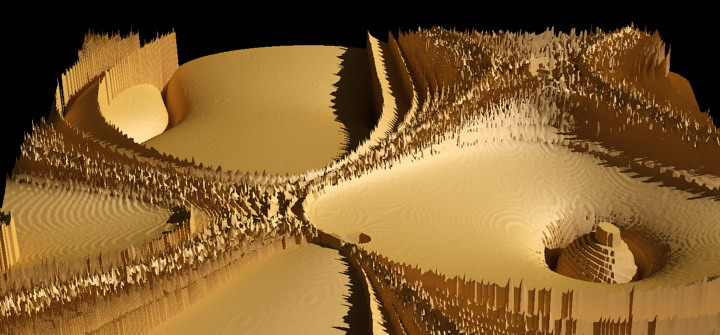
\includegraphics[width=0.32\linewidth]{imgs/tp04a_450}
 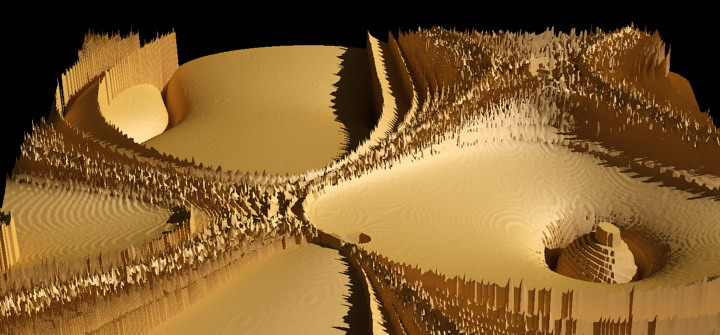
\includegraphics[width=0.32\linewidth]{imgs/tp04a_450}
 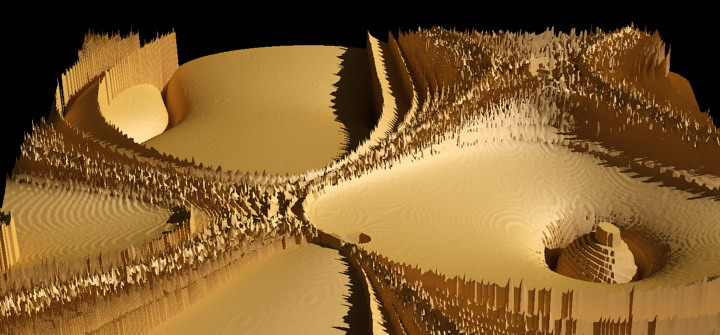
\includegraphics[width=0.32\linewidth]{imgs/tp04a_450}
 % tp04a_450.jpg: 720x335 pixel, 72dpi, 25.40x11.82 cm, bb=0 0 720 335
 \caption[curta]{Imagem composta por três figuras em ficheiros separados}
 \label{fig:terrenos}
\end{figure}


\begin{figure}
 \centering
 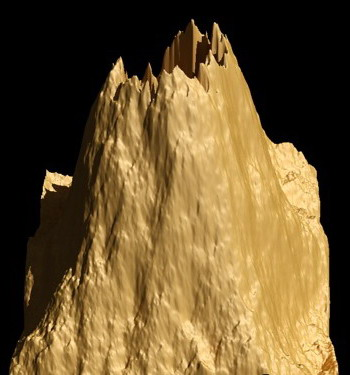
\includegraphics[width=0.5\linewidth]{imgs/tp45a_450}
 % tp45a_450.eps: 1179666x1179666 pixel, 300dpi, 9987.84x9987.84 cm, bb=20 20 575 615
 \caption{Vulcão}
 \label{fig:volcao}
\end{figure}


Na Tabela \ref{tableBenchmark} temos um exemplo de uma tabela onde existem linhas que ocupam mais do que uma linha da tabela.

% TODO - falta fazer isto!

\begin{table}
  \caption[exemplo de uma tabela]{Floating point benchmark.
	\textbf{R$_{max}$}: the performance in Gflops for the largest problem run on a machine;
	\textbf{N$_{max}$}: the size of the largest problem run on a machine;
	\textbf{N$_{1/2}$}: the size where half the R$_{max}$ execution rate is achieved;
	\textbf{R$_{peak}$}: the theoretical peak performance in Gflops for the machine}
  \label{tableBenchmark}
  \begin{center} 
  \begin{tabular*}{1\textwidth}{@{\extracolsep{\fill}} rccccc } \toprule
\textbf{Linpack	Benchmark}& Proc.	& \textbf{R$_{max}$} & \textbf{N$_{max}$} & \textbf{N$_{1/2}$}	& \textbf{R$_{peak}$} \\ 
(Full precision)	& or Cores	& GFlops	     & Order		  & Order		& GFlops \\ [0.25ex] \midrule
Thinking Machine CM-5	& 32		& 1,900		     & 9216		  & 4096		& 4 \\
Pentium 4 3.0 GHz & 1	& 4,730		     & 7600		  & 365			& 6 \\
\multirow{2}{*}{IBM Cell BE 3.2 GHz} 	& \multirow{2}{*}{9}& \multirow{2}{*}{98,05} & \multirow{2}{*}{4096} & \multirow{2}{*}{1536} & 204,8 {\scriptsize{(32 bits)}} \\
			&		&		     &			  &			& 14,6 {\scriptsize{(64 bits)}} \\ \bottomrule
  \end{tabular*}
  \end{center}	
\end{table}



As técnicas evolutivas baseiam-se em algoritmos bio-inspirados que aplicam a teoria de Darwin \parencite{Darwin1859}. Esta defende a evolução natural das espécies onde os organismos vivos são recompensados, através da sobrevivência e da propagação dos seus próprios genes aos sucessores. Actualmente existem quatro classes principais de algoritmos evolutivos: Algoritmos Genéticos (AG) \parencite{Holland1975}, Estratégias Evolutivas, Programação Genética (GP) \parencite{Koza1992} e Programação Evolutiva. Todos os algoritmos evolutivos mantêm uma população de soluções candidatas sobre a qual efectuam uma pesquisa para determinar os indivíduos mais fracos. De acordo com um determinado critério, estes são substituídos por outros gerados através de operadores aplicados aos melhores indivíduos da população, criando assim uma nova geração. Este processo é repetido sobre sucessivas gerações até se encontrar uma boa solução, que pode não ser a óptima.

Existem vários trabalhos e até video jogos que usam algoritmos evolutivos \parencite{Sims1992,url_Spore}.

\section{Incluir código fonte}
Nas Listagens \ref{ls:fibonacci} e \ref{ls:bash} temos um exemplo da inclusão de código fonte diretamente a partir do ficheiro fonte. Para mais informação ler o Manual da packge minted \parencite{Rudolph2016}. Nestes exemplos a formação foi configurada no ficheiro \texttt{config.tex} (procurar por \texttt{minted}). 


\begin{listing}[H] % quando cabe numa só página
    \caption{Código fonte C com sintaxe colorida}
    \label{ls:fibonacci}
    \codefilec{Code/fibonacci.c}
\end{listing}


\begin{longlisting} % quando ocupa mais que uma página
    \caption{Código fonte Bash que ocupa \underline{mais que uma página}}
    \label{ls:bash}
    \codefilebash{Code/bash.sh}
\end{longlisting}



Também é possível incluir código diretamente no ficheiro \LaTeXe, como no exemplo em baixo. A numeração das linhas é importante para ser possível referir o número da linha numa descrição.



\begin{listing}[H]
    \caption{Código fonte Python com sintaxe colorida}
    \label{ls:bash}
    \begin{pythoncode}
import numpy as np

def incmatrix(genl1,genl2):
    m = len(genl1)
    n = len(genl2)
    M = None #to become the incidence matrix
    VT = np.zeros((n*m,1), int)  #dummy variable

    #compute the bitwise xor matrix
    M1 = bitxormatrix(genl1)
    M2 = np.triu(bitxormatrix(genl2),1) 

    for i in range(m-1):
        for j in range(i+1, m):
            [r,c] = np.where(M2 == M1[i,j])
            for k in range(len(r)):
                VT[(i)*n + r[k]] = 1;
                VT[(i)*n + c[k]] = 1;
                VT[(j)*n + r[k]] = 1;
                VT[(j)*n + c[k]] = 1;

                if M is None:
                    M = np.copy(VT)
                else:
                    M = np.concatenate((M, VT), 1)

                VT = np.zeros((n*m,1), int)

return M
    \end{pythoncode}
\end{listing}

\cleardoublepage\addtocontents{toc}{\protect\vspace{\beforebibskip}} % Place slightly below the rest of the document content in the table


%************************************************
\chapter{Conclusões}
\label{ch:conclusoes}
%************************************************


O uso do \LaTeXe permite-nos focar no essencial: o conteúdo, a formatação é tratada de forma automática.

Para mais informações sobre o \LaTeXe aconselha-se a consulta do
livro \emph{The Not So Short Introduction to \LaTeXe}~\cite{oetiker2000nss}.

Para a gestão de referências bibliográficas aconselha-se o JabRef. %\cite{jabref}.
 

\cleardoublepage%********************************************************************
% Bibliography
%*******************************************************
% work-around to have small caps also here in the headline
\manualmark
\markboth{\spacedlowsmallcaps{\bibname}}{\spacedlowsmallcaps{\bibname}} % work-around to have small caps also
\phantomsection 
\refstepcounter{dummy}
\addtocontents{toc}{\protect\vspace{\beforebibskip}} % to have the bib a bit from the rest in the toc
\addcontentsline{toc}{chapter}{\tocEntry{\bibname}}

\printbibliography
\label{app:bibliography} 


%********************************************************************
% Backmatter
%*******************************************************
\appendix

\cleardoublepage
\phantomsection 
\part*{Apêndices}

\cleardoublepage\addtocontents{toc}{\protect\vspace{\beforebibskip}} % Place slightly below the rest of the document content in the table

% If problems with the headers: get headings in appendix etc. right
\markboth{\spacedlowsmallcaps{Anexos}}{\spacedlowsmallcaps{Anexos}}

% Appendix A
\chapter{Apêncice A}

%----------------------------------------------------------------------------------------

\lipsum[13-14]

%----------------------------------------------------------------------------------------

\section{Appendix Section Test}
\lipsum[15]

\lipsum[16]

%----------------------------------------------------------------------------------------

\section{Another Appendix Section Test}
\lipsum[17]

\begin{table}
\myfloatalign
\begin{tabularx}{\textwidth}{Xll} \toprule
\tableheadline{labitur bonorum pri no} & \tableheadline{que vista}
& \tableheadline{human} \\ \midrule
fastidii ea ius & germano &  demonstratea \\
suscipit instructior & titulo & personas \\
\midrule
quaestio philosophia & facto & demonstrated \\
\bottomrule
\end{tabularx}
\caption[Autem usu id]{Autem usu id.}
\label{tab:moreexample}
\end{table}

\lipsum[18]





\cleardoublepage\addtocontents{toc}{\protect\vspace{\beforebibskip}} % Place slightly below the rest of the document content in the table

% Appendix X
\chapter{Apêncice B}
%----------------------------------------------------------------------------------------

% Content begins here


\lipsum[15]



\cleardoublepage%*******************************************************
% Declaration
%*******************************************************


\refstepcounter{dummy}
\addtocontents{toc}{\protect\vspace{\beforebibskip}} % to have the bib a bit from the rest in the toc
\addcontentsline{toc}{chapter}{\tocEntry{Declaração}}
\chapter*{Declaração}
\thispagestyle{empty}


Declaro, sob compromisso de honra, que o trabalho apresentado nesta dissertação, com o título \textit{``\myTitle''}, é original e foi realizado por \myNameOne (\myNumber) sob orientação de \myProfOne.

\vspace{15 mm}

\noindent\textit{\myLocation, \myTime}
\bigskip

\begin{flushright}
    \begin{tabular}{m{8cm}}
        \\ \hline
        \centering\myNameOne \\
    \end{tabular}
\end{flushright}

% \vspace{5 mm}
% 
% \begin{flushright}
%     \begin{tabular}{m{8cm}}
%         \\ \hline
%         \centering\myNameTwo \\
%     \end{tabular}
% \end{flushright}




% 
% \begin{flushright}
%     \begin{tabular}{|m{10cm}}
%         \\ 
%         \centering  %\myName \\
%     \end{tabular}
% \end{flushright}
% 
% \vspace{5 mm}
% \begin{flushright}
%     \begin{tabular}{|m{10cm}}
%         \\ 
%         \centering  %\myName \\
%     \end{tabular}
% \end{flushright}
% 
% 

%********************************************************************
% Game Over: Restore, Restart, or Quit?
%*******************************************************
\end{document}
%********************************************************************
